\section{Video Synthesis}
\label{sec:video_synthesis}

% \begin{figure}
%     \centering
%     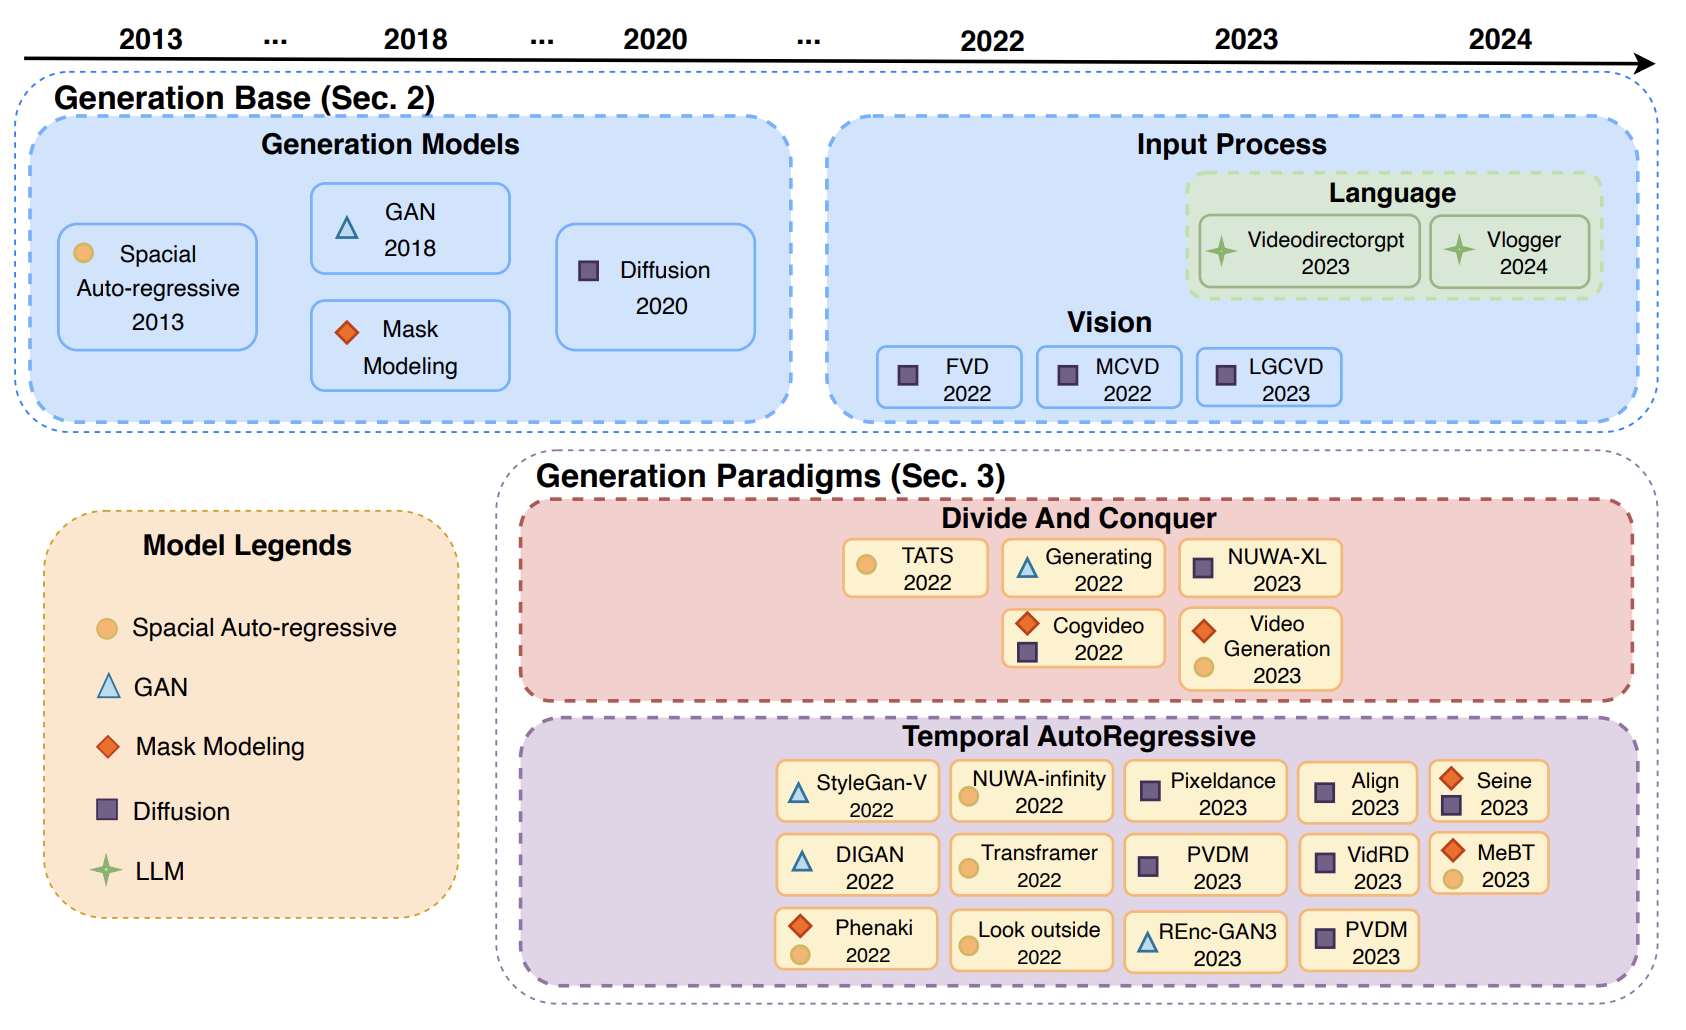
\includegraphics[width=0.7\textwidth]{images/video_synthesis/techniques.png}
%     \caption{Overview of video synthesis techniques \cite{long_video_survey}.}
%     \label{fig:video_synthesis_techniques}
% \end{figure}

Video synthesis is a complex task. One can think of video generation as a sequence of image generation tasks. Formally, a video is a sequence of images (or frames) that are shown in fast fashion, usually 24 frames per second (at the minimum, to get smooth video). Therefor to create a smooth video of 5 seconds, you'll need 120 frames or images at the minimum. Video data is complex; we have the addition of the \textbf{time dimension}, which is not present in image generation tasks. The video should be \textbf{coherent} in time, meaning that the frames should be related to each other and should follow a logical sequence. Objects should not appear out of nowhere, there should be \textbf{smooth transition of motion} and correct \textbf{spatial relationships} between objects. We also have to deal with limited hardware resources, since video generation is extremely computationally expensive.

% TODO: Add timeline of video synthesis models
% \begin{figure}
    \centering
    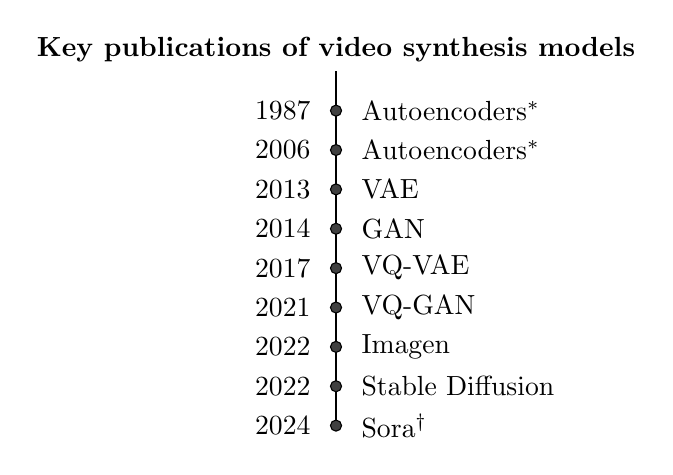
\begin{tikzpicture}
        \def\step{0.5} % step size for vertical spacing
        \def\numtimeline{9} % Number of events in the timeline

        % Define timeline line
        \draw[thick, color=black] (0,0) -- (0,-\numtimeline*\step);

        % Define timeline events with adjusted positions
        \foreach \i/\year/\text in 
        {
            1/1987/Autoencoders$^*$, 
            2/2006/Autoencoders$^*$, 
            3/2013/VAE, 
            4/2014/GAN, 
            5/2017/VQ-VAE,
            6/2021/VQ-GAN,
            7/2022/Imagen,
            8/2022/Stable Diffusion,
            9/2024/Sora$^\dag$
        } {
        \draw[fill=darkgray] (0,-\i*\step) circle (2pt);
        \node[anchor=east] at (-0.2,-\i*\step) {\year};
        \node[anchor=west] at (0.2,-\i*\step) {\text};
        }

        % Define timeline title
        \node[anchor=south] at (0,0) {\textbf{Key publications of video synthesis models}};
    \end{tikzpicture}
    \caption{Chronology of key video generation models publications.}
  \end{figure}

% There are a lot of techniques and models for video generation, and they can be divided into multiple categories:

% \begin{itemize}
%     \item \textbf{Frame prediction}: ...
%     \item \textbf{GAN based models}: such in the case of \cite{chu2020learning} the authors propose 
% \end{itemize}

Video synthesis can be based on four main methods:

\begin{enumerate}
    \item \textbf{Diffusion}: diffusion models for video generation extend the iterative refinement process used in image-based diffusion models, such as LDMs, to handle temporal dynamics required for videos. The key idea is to generate not just a sequence of independent images, but a continuous video where both the spatial content of each frame and the temporal coherence between frames are learned and generated simultaneously.
    \item \textbf{Spatial autoregressive}: spatial autoregressive models for video generation, as described in \cite{graves2013generating}, synthesize video by sequentially generating content in a patch-based fashion, where each patch in a frame is conditioned on previously generated patches. This method builds video frame-by-frame, ensuring spatial and temporal coherence.
    \item \textbf{GAN}: similar to diffusion models, GANs can also be leveraged for video synthesis. However, it's used seldom because of unstable training, partly due to the adversarial loss objective.
    \item \textbf{Mask modeling}: mask modeling in video generation uses the technique of selectively masking parts of video frames. The model is tasked with predicting and reconstructing the missing parts, forcing it to better understand the underlying structure and motion in the video.
\end{enumerate}

\begin{figure}
    \centering
    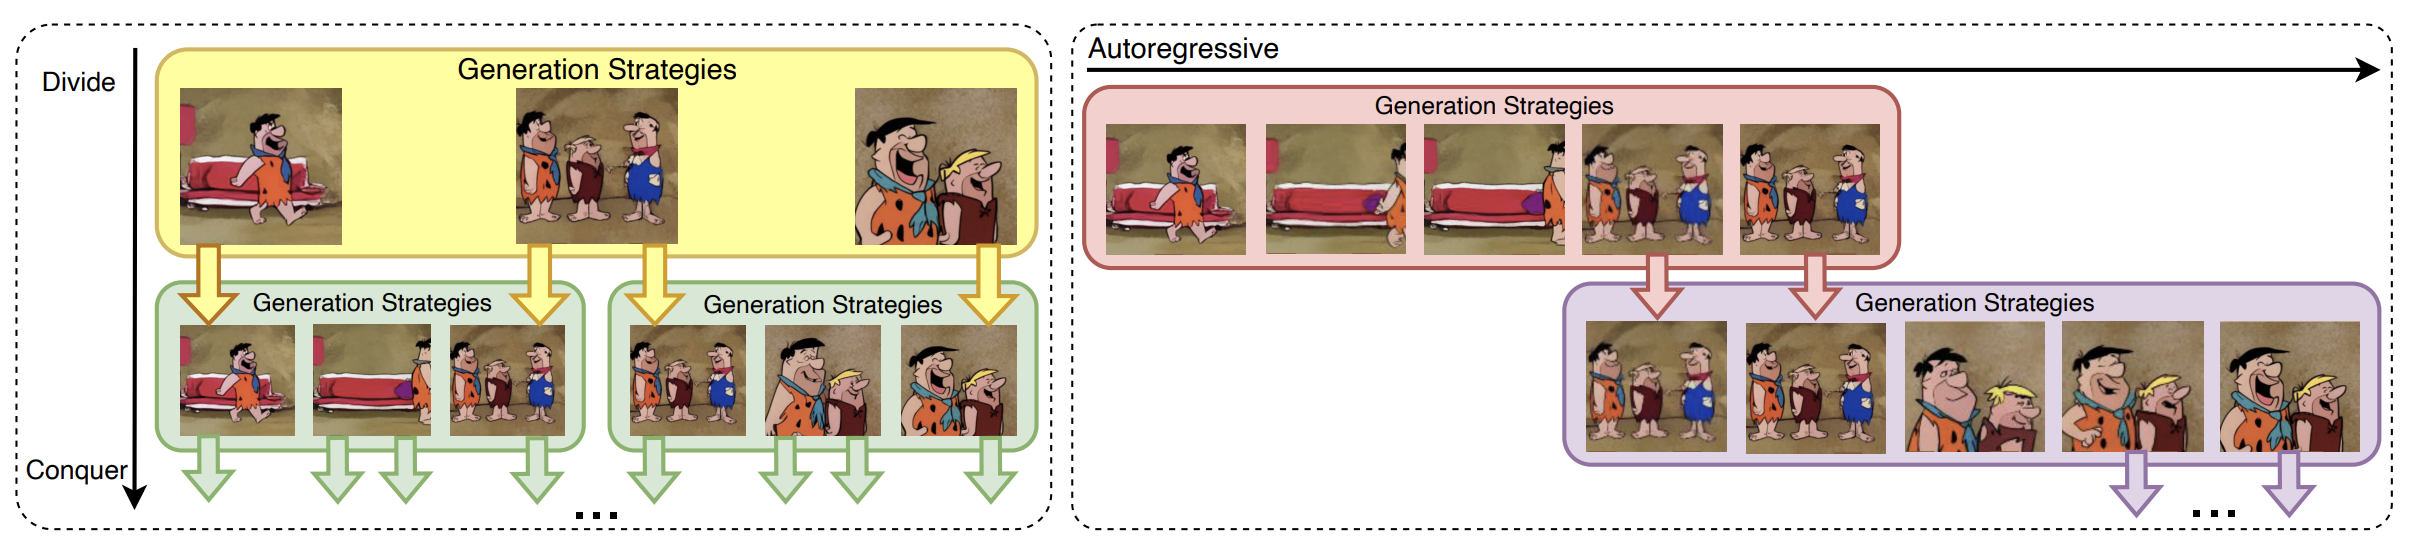
\includegraphics[width=0.9\textwidth]{images/video_synthesis/paradigms.png}
    \caption{Overview of video synthesis paradigms \cite{long_video_survey}. Divide and conquer is split into hierarchical architecture for keyframe generation and frame filling. Whereas temporal autoregressive paradigm the next frame prediction depends on the previous frame/frames \cite{long_video_survey}.}
    \label{fig:video_synthesis_paradigms}
\end{figure}

In the realm of video synthesis there are two paradigms: \textbf{divide and conquer} and \textbf{temporal autoregressive}. An overview of the paradigms is shown in figure \ref{fig:video_synthesis_paradigms}.


\begin{figure}
    \centering
    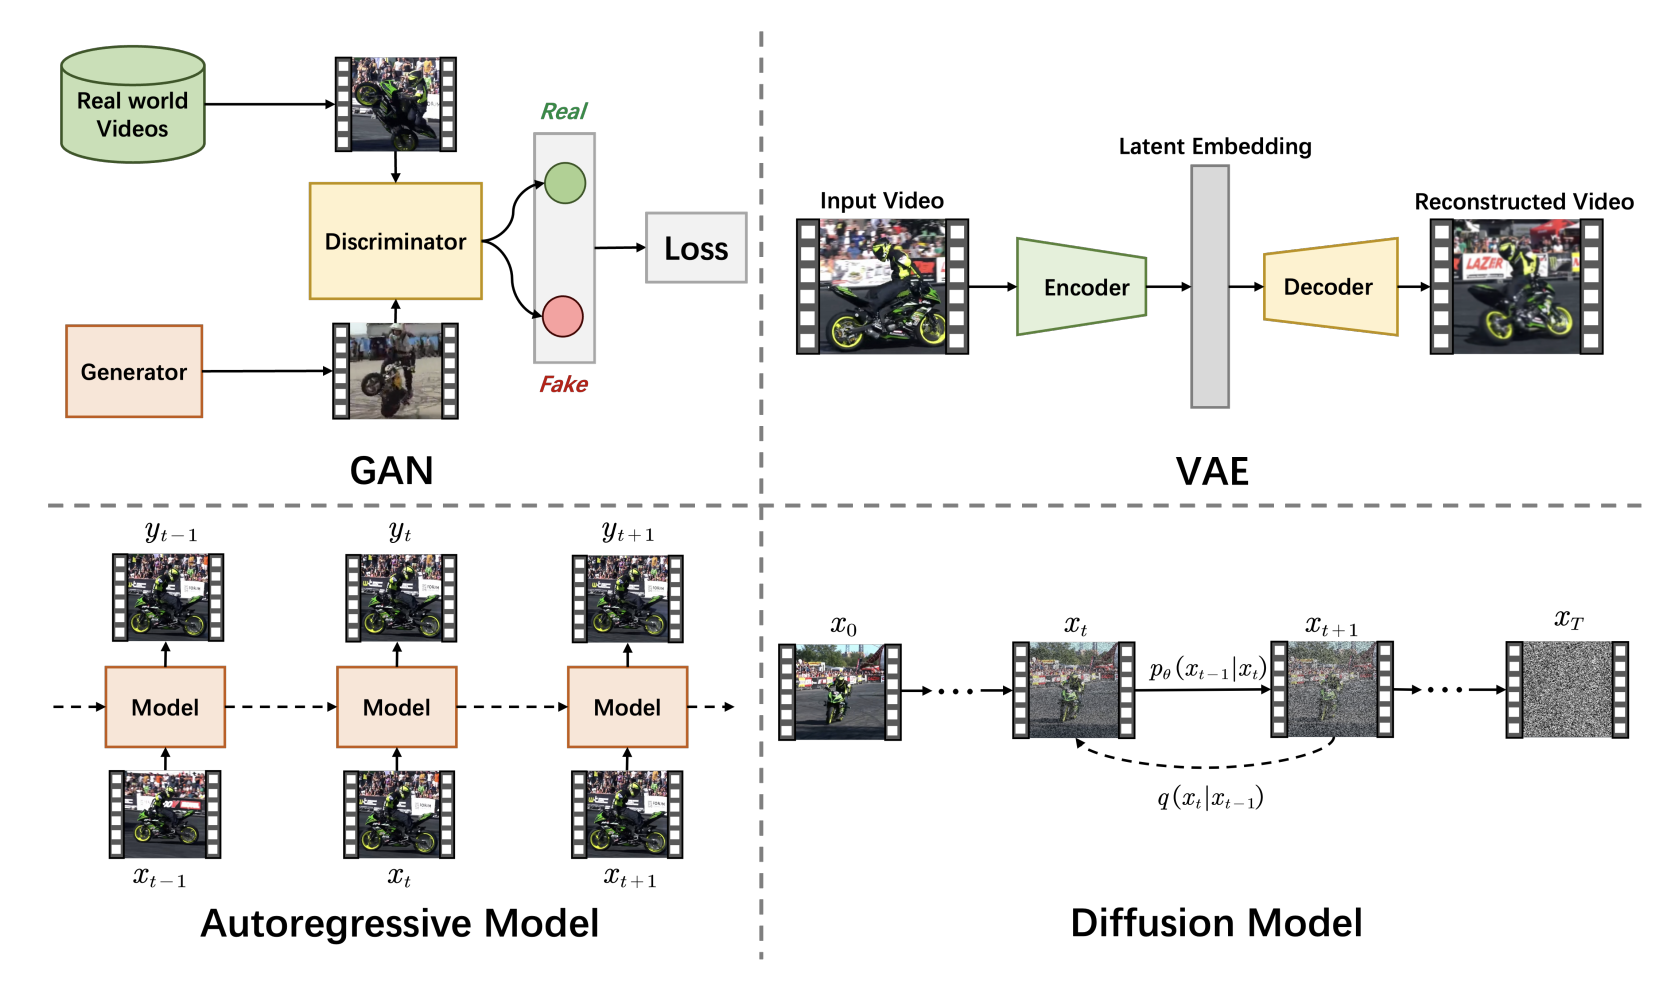
\includegraphics[width=0.6\textwidth]{images/video_synthesis/generation_technologies.png}
    \caption{Overview of video generation technologies \cite{zhou2024survey}.}
    \label{fig:video_synthesis_generation_technologies}
\end{figure}

In figure \ref{fig:video_synthesis_generation_technologies} we can see different video generation techniques, some we already covered: GAN, VAE, diffusion and autoregressive. The autoregressive model we did not yet covered; it is covered in the next sections.








\subsection*{Temporal autoregressive}

Temporal autoregressive paradigm is an iterative approach where each frame is generated based on the previous one (or previous multiple frames). The model is trained on sequences of video data, and the output from one timestep serves as the input for the next (the next frame is conditioned on the previous frame, which in theory ensures that the video is temporally coherent).

A significant amount of research has been conducted on temporal autoregressive models, leading to various improvement strategies and enhancements for this framework. Some of the most notable include:

\begin{itemize}
    \item \textbf{Latent space compression}: this method focuses on compressing videos to latent space to optimize computational needs. For example in \cite{zeng2024make} and \cite{gu2023reuse} they explored condensing video data into 3D latent. Compression aims to preserve essential features across dimensions to improve computational efficiency.
    \item \textbf{Incorporating temporal layers} to refine individual video clips. Advancements were made, such as integrating \textbf{temporal layers} such as attention and convolutional layers into diffusion models, like in VideoLDM \cite{video_ldm} and \cite{gu2023reuse}. These temporal layers help the model better understand the temporal dynamics of video data.
    \item \textbf{Dual-phase training \& reuse strategies}: dual-training is a training strategy where the model is first trained unconditionally, and then learn to conditionally generate video like in Projected Latent Video Diffusion Model (PVDM) \cite{pvdm}. Given the abundance of unlabeled video data on the web, it's easy to see why this process is attractive. Another method to boost the model's ability to replicate long video sequences is a \textbf{reuse strategy}, which iteratively adds and removes noise during training to simulate natural variability, like in \cite{gu2023reuse}.
\end{itemize}








\subsection*{Divide and Conquer}

Divide and conquer paradigm breaks the task of video synthesis into smaller, more manageable tasks. This approach can further by divided into 3 methods of approach:

\begin{enumerate}
    \item \textbf{Hierarchical architecture for frame generation}: in this approach, the process is split into \textbf{keyframe generation} and \textbf{frame filling} models. Keyframes represent the critical moments of the video that establish the narrative, while the frame-filling models ensure smooth transitions between them. Global models focus on generating the main storyline through keyframes, and local models handle finer details, filling the gaps between the keyframes to maintain temporal consistency.
    \item \textbf{Multi-stage approach for video super-resolution}: \cite{brooks2022generating} suggested generating video by stages, first by creating low-resolution sequences with GAN and then applying super-resolution models to enhance them with StyleGAN3 \cite{stylegan3}.
    \item \textbf{Integrated keyframe and frame filling with mask modeling} simplifies long video generation by combining keyframe creation and frame filling into a unified process. Mask modeling hides specific parts of the video during training, keyframes and intermediate frames simultaneously, like done in CogVideo \cite{cogvideo}, which simplified mask modeling and combines these models into a single model.
\end{enumerate}














\subsection*{Spatial autoregressive models}

Spatial autoregressive models are adept at processing tokenized sequence inputs (they include the transformer architecture) which enable the segmentation of video frames into patches. By integrating video data features with the autoregressive power of transformers, these models become more capable of capturing temporal dynamics. In this method, there are two main approaches:

\begin{itemize}
    \item \textbf{Frame tokenization}: like in NUWA-Infinity \cite{nuwa_infinity}, where video frames are transformed into patches, and each patch is projected to a patch embedding, and combine them with spatial positional encodings. These autoregressive models, similar to LDMs, compress video into latent space. Compression techniques like \textbf{Discrete Cosine Transform (DCT)} are used in Transframer \cite{transframer} framework and by using a VQ-GAN, they convert the frames into latent tokens.
    \item \textbf{Scaling with attention mechanism}: architectural modifications were made by incorporating specialized blocks, such as attention mechanism blocks tailored for spatiotemporal data. For example, Transframer \cite{transframer} integrated temporal and spatial annotations (time-steps, camera viewport, etc.) through cross-attention.
\end{itemize}















\subsection{Evaluation metrics}

\begin{figure}
    \centering
    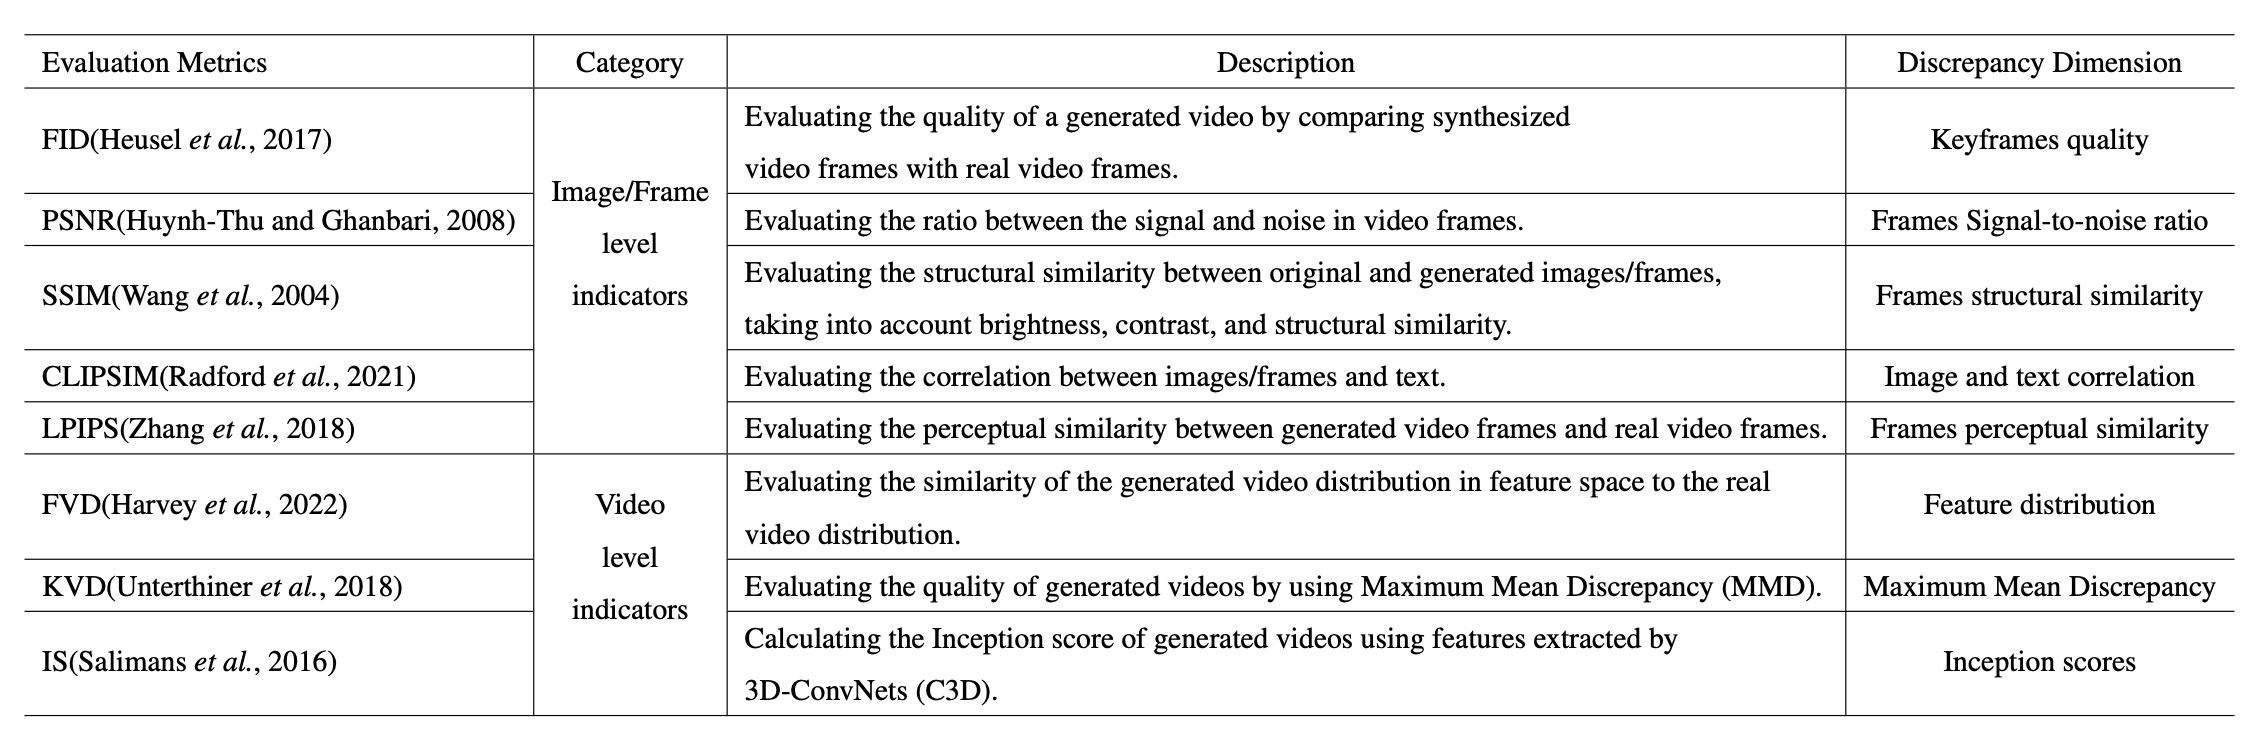
\includegraphics[width=1\textwidth]{images/video_synthesis/eval_metrics.png}
    \caption{Evaluation metrics in video generation \cite{long_video_survey}.}
    \label{fig:video_synthesis_eval_metrics}
\end{figure}

A common metric used for video generation models is the \textbf{Frechet Video Distance (FVD)} \cite{fvd}, which is an extension of Frechet Inception Distance (FID). FVD compares videos by both spatial and temporal features by using similar process as FID: using a pre-trained 3D ConvNet (i3D), where in FID they use InceptionV3. In similar fashion as FID, FVD compares the distribution of features of video clips:

\begin{equation*}
    \text{FVD} = \left| \left| \mu_{\text{real}} - \mu_{\text{fake}} \right| \right|^2_2 + \text{Tr} \left( \Sigma_{\text{real}} + \Sigma_{\text{fake}} - 2 \left( \Sigma_{\text{real}} \Sigma_{\text{fake}} \right)^{1/2} \right)
\end{equation*}

where $\mu_{\text{real}}$, $\mu_{\text{fake}}$ is the mean of the real and fake data, $\Sigma_{\text{real}}$, $\Sigma_{\text{fake}}$ is the covariance matrix of the real and fake data, $\text{Tr}$ function is the trace of the matrix, and $\left| \left| \cdot \right| \right|^2_2$ is the squared Euclidean norm.

The lower the FVD score, the better the video generation model. A more comprehensive list of evaluation metrics is shown in figure \ref{fig:video_synthesis_eval_metrics}.

In the Diffusion Transformer (DiT) paper \cite{diffusion_transformer} the researchers used \textbf{Gflops} (giga floating point operations per second) metric to measure the complexity of the model, instead of traditional parameter count of the model. Higher Gflops means the model is more scalable and complex.








\subsection{Previous works}

\begin{figure}
    \centering
    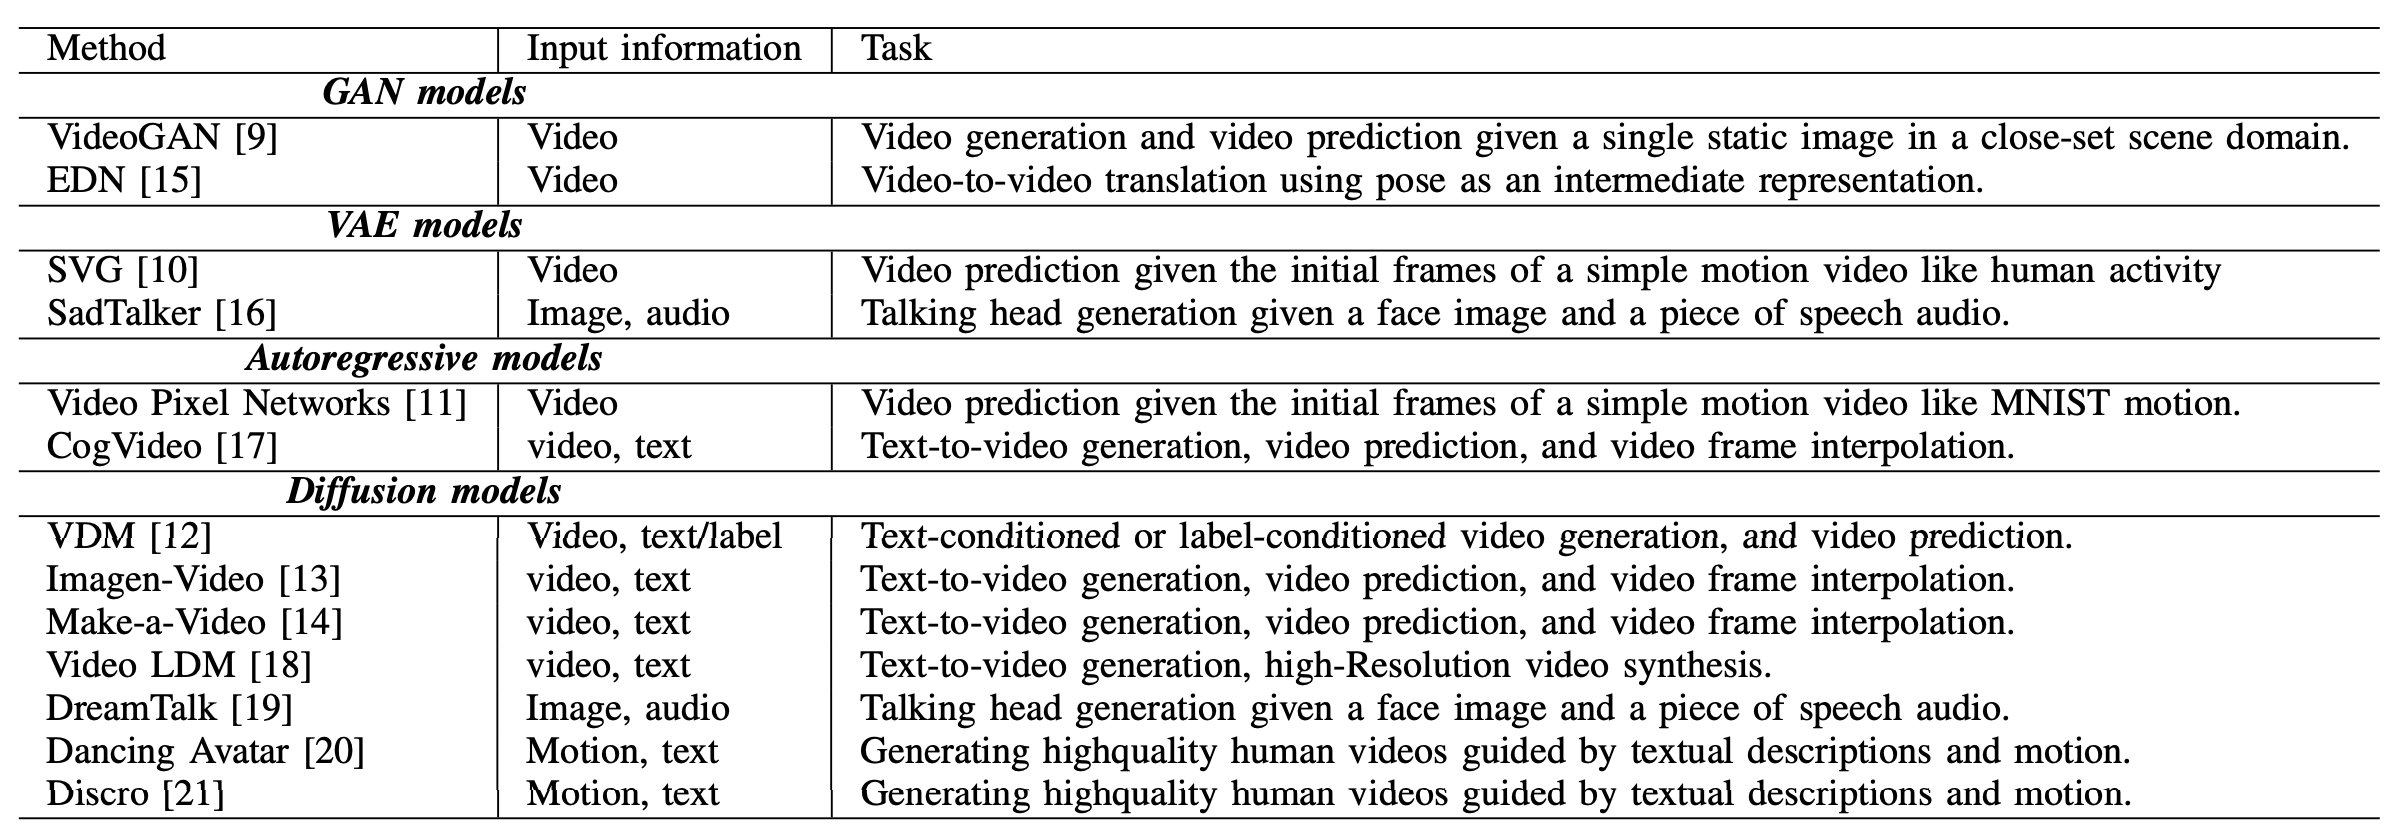
\includegraphics[width=0.7\textwidth]{images/video_synthesis/previous_works.png}
    \caption{Video generation models \& papers \cite{zhou2024survey}.}
    \label{fig:video_synthesis_previous_works}
\end{figure}

In figure \ref{fig:video_synthesis_previous_works} we can see different models, divided into four main categories (VAE, GAN, diffusion, autoregressive) for the task of video synthesis. Different models have different input methods (video, text, audio, motion, etc.).

\begin{figure}
    \centering
    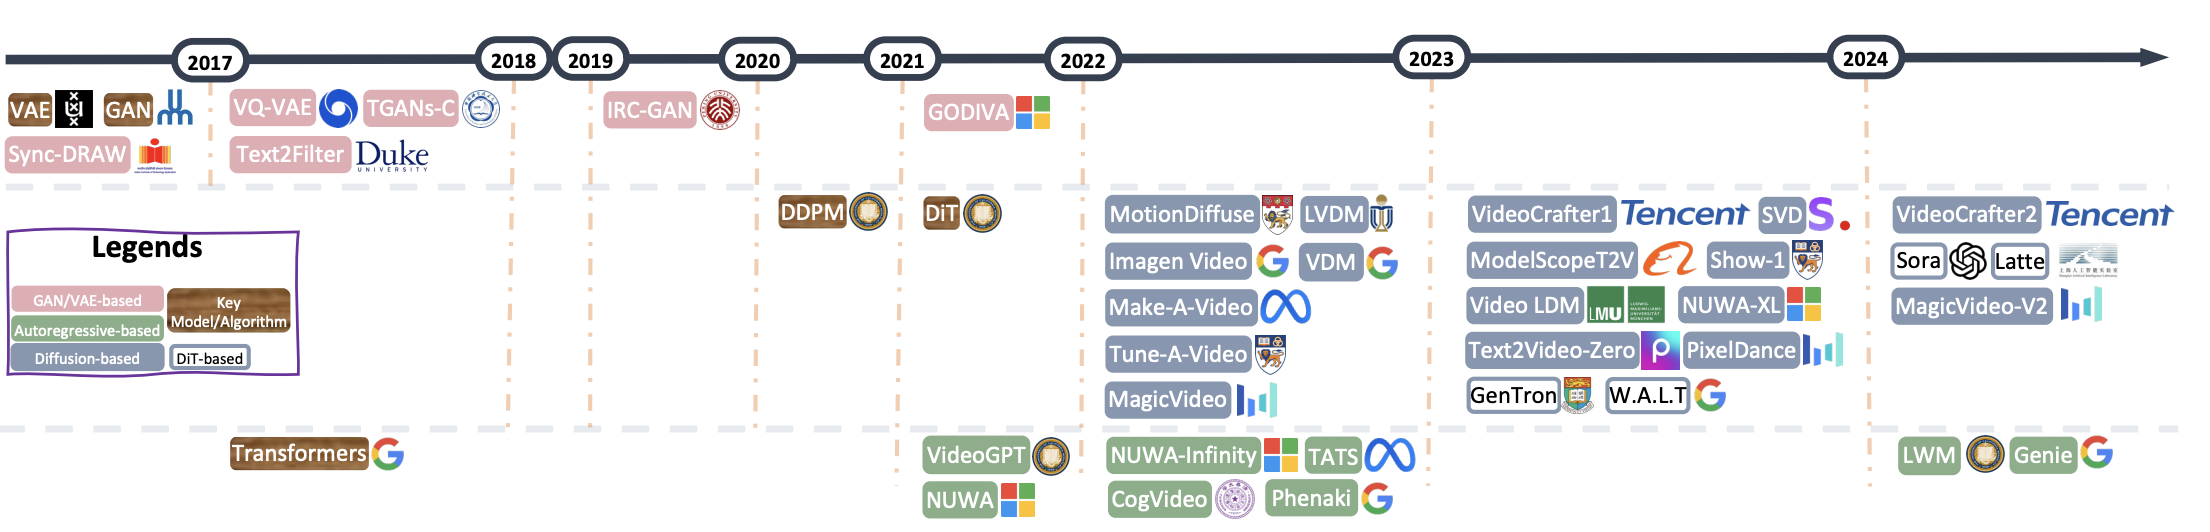
\includegraphics[width=0.9\textwidth]{images/video_synthesis/timeline.png}
    \caption{Text-to-Video generators evolutionary timeline, based on foundational algorithms \cite{sun2024sora}.}
    \label{fig:video_synthesis_timeline}
\end{figure}

In figure \ref{fig:video_synthesis_timeline} we can see the timeline of different text-to-video models, their paper origin (Meta, Microsoft, Google, OpenAI, and even some universities) based on foundational algorithms (GAN/VAE, Autoregressive, Diffusion and Diffusion Transformer). We can also see the key models/algorithms, such as transformers, DDPM, DiT, and more.

\textbf{NUWA-Infinity } \cite{nuwa_infinity}, introduced by Microsoft AI in 2022, is a T2V model capable of generating videos of arbitrary resolution and length. It ensures spatial and temporal consistency through an innovative \textbf{autoregressive over autoregressive} generation mechanism. This mechanism combines two levels of autoregressive modeling: a global patch-level model that captures dependencies between patches and a local token-level model that addresses dependencies within visual tokens of each patch.

\textbf{NUWA-XL} \cite{nuwa_xl} (2023, which is an upgraded version of NUWA-Infinity) is a diffusion T2V model that uses a 3D U-Net in global model for keyframe generation and a model for keyframe filling. They also built a new dataset called 'FlintstonesHD' for benchmarking long video generation. Their method reduced inference time when generating 1024 frames from 7.55 minutes to 26 seconds (\textbf{a 94\% reduction in inference time}) on the same hardware.

\textbf{Image-GPT (iGPT)}: OpenAI's 2020 paper introduced Image-GPT \cite{imagegpt}, an autoregressive image generation transformer model that predicts pixels directly using attention mechanisms. Pre-trained on ImageNet, iGPT demonstrated the ability to learn spatial features for image representation.

\textbf{Video Diffusion Models (VDM)}: Google's 2022 work \cite{video_diffusion_models} extended image diffusion models to video generation using a 3D U-Net architecture. They replaced 2D convolutions with space-only 3D convolutions and introduced temporal attention blocks alongside spatial ones. Relative position embeddings were used to capture frame order, enabling the model to handle both images and videos.

\textbf{MagicVideo} (2022) \cite{magic_video} from ByteDance is a T2V model leverage LDM based on 3D U-Net and a directed temporal attention, and a pre-trained VAE to map video clips to low-dimension latents to learn the distribution of the latent codes. It is based on keyframe and frame filling paradigm and uses CLIP to encode the text prompt.

\textbf{CogVideo} (2022) \cite{cogvideo} is a 9 billion parameters open-source video synthesis model that is based on CogView2, which is a T2I model. It uses an autoregressive transformer, that works in latent space to generate video frames. CogVideo also lists VideoGPT as related work, and upgrades upon it.

\textbf{EasyAnimate}: Alibaba's 2024 multi-modal diffusion video generation model \cite{easyanimate} uses a 12-billion-parameter Diffusion Transformer (DiT) (appendix \ref{appendix:diffusion_transformer}) to scale attention mechanisms to the video domain. It introduces Slice VAE, which reduces GPU memory usage compared to traditional video VAEs.

\textbf{To summarize}: Researchers agree that generating high-cohesion, long videos requires modeling long-range temporal dependencies. GANs are challenging to optimize for video tasks due to adversarial loss, unlike the likelihood loss used in VAEs, diffusion models, and transformers. And finally, they agree that:

\begin{quote}
    \textit{"... the video domain has not yet witnessed its 'AlexNet moment'"} \cite{tran2018closer}
\end{quote}

AlexNet \cite{alexnet} was a major breakthrough in 2012 for image classification task which led to the development of imaging domain in deep learning.










\subsection{Spatiotemporal feature learning}

One of the first work that tries to capture temporal dynamics is in a form of sequence-to-sequence video captioning \cite{venugopalan2015sequence} (2015). In this paper, the researchers used \textbf{Long Short-Term Memory model (LSTM)} to caption video, which was a popular model for sequence tasks at that time (and also Recurrent Neural Networks [RNN] which was prior work to LSTMs). However, LSTMs struggled with issues like exploding/vanishing gradients, leading to their replacement by more scalable models.

Modern approaches leverage 3D convolution networks (3D ConvNets) and temporal attention. A 2014 paper \cite{tran2015learning} by Facebook AI introduced 3D ConvNets for spatiotemporal feature learning. The researchers found that 3x3x3 kernel size is the best option for 3D ConvNets. After every convolution layer they apply 3D max-pooling.

Figure \ref{fig:c3d_feature_maps} shows the feature maps of the first 3D convolution layer of the C3D model \cite{tran2015learning}.

And in figure \ref{fig:video_synthesis_3d_conv} we can see how 3D convolution evolved from 1D and 2D convolution. The output of 2D convolution flat (2D), compared to 3D convolution where we also have volume, which is used as the frames dimension in video synthesis models.

\begin{figure}
    \centering
    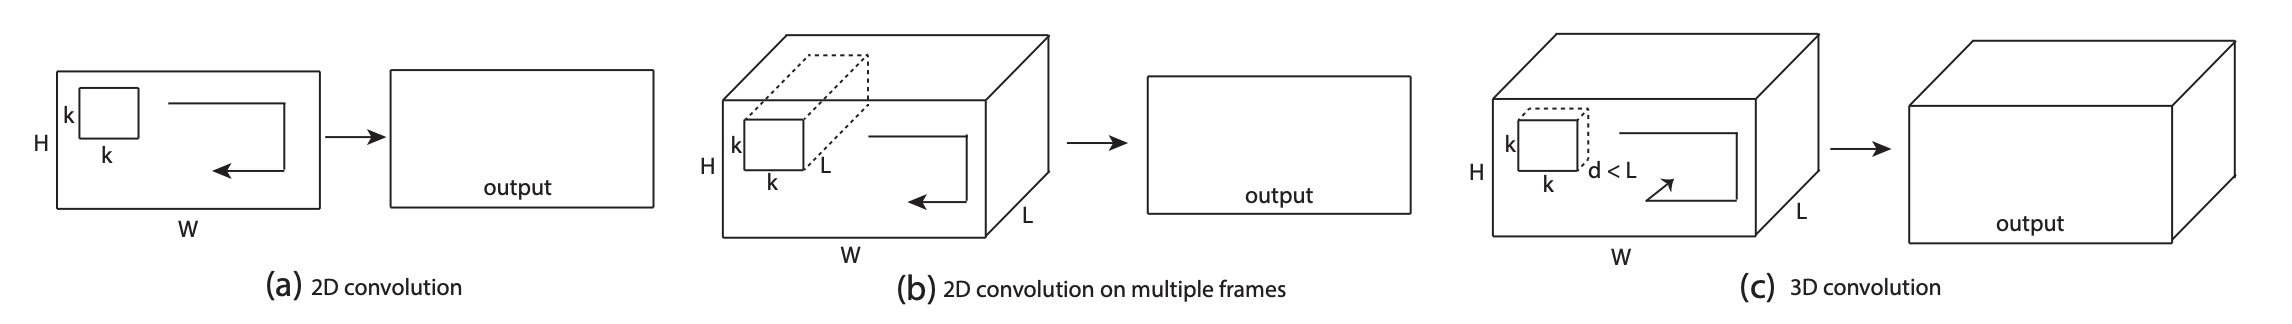
\includegraphics[width=0.7\textwidth]{images/video_synthesis/conv.png}
    \caption{2D and 3D convolution operations. (a) Applying 2D convolution on image results in an image. (b) Applying 2D convolution on video (multiple frames) also results in an image. (c) Applying 3D convolution on video results in another volume (channel), preserving temporal information \cite{tran2015learning}.}
    \label{fig:video_synthesis_3d_conv}
\end{figure}

\begin{figure}
    \centering
    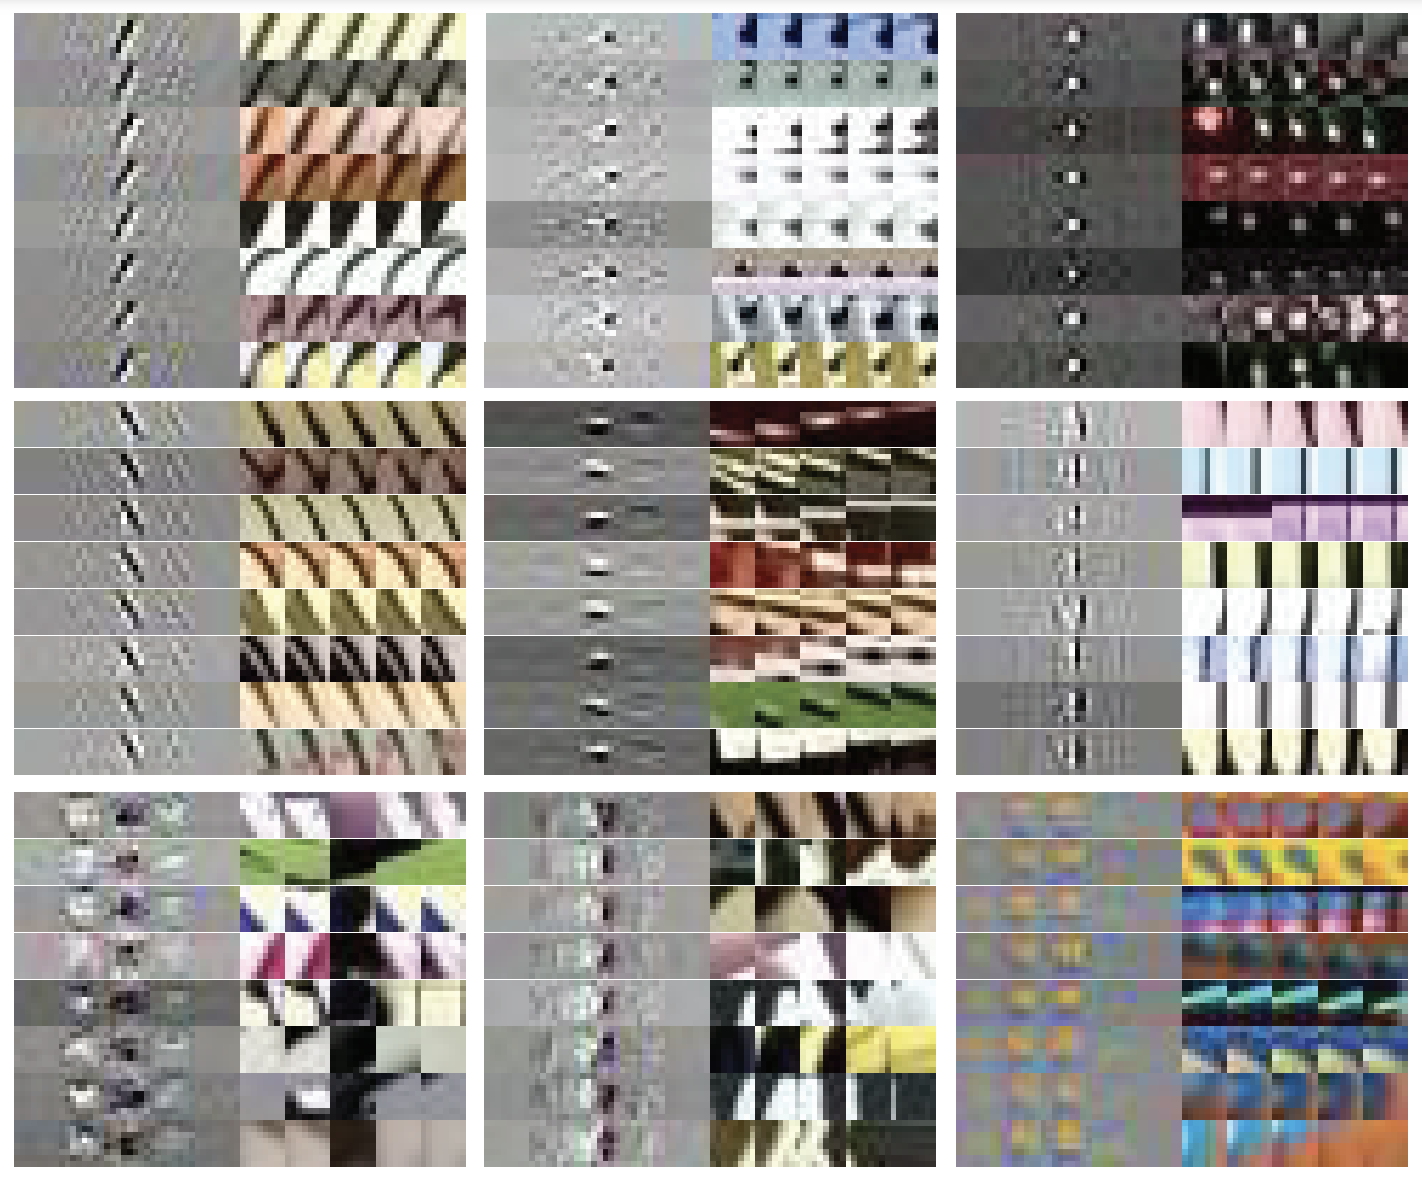
\includegraphics[width=0.5\textwidth]{images/video_synthesis/c3d_feature_maps.png}
    \caption{Feature maps of the first 3D convolution layer of the C3D model \cite{tran2015learning}. The first two rows of the feature maps shows the detection of moving edges and blobs, while the last row shows edge orientation changes and color changes \cite{tran2015learning}.}
    \label{fig:c3d_feature_maps}
\end{figure}

Further improvements in a 2018 paper \cite{tran2018closer} also by Facebook AI proposed R(2+1)D blocks, separating spatial and temporal convolutions into a 2D residual block followed by a 1D temporal convolution. This structure enhanced optimization and enabled modeling of complex non-linear functions, making it a strong performer for action recognition.














\subsection{Practices \& techniques in vision domain}

In this section we explore common practices or techniques used in vision domain, that are applied in image synthesis and video synthesis models.

\textbf{Use of transformers for multi-modal outputs:} Transformers have been shown time and time again their capability to scale very well given large enough datasets. In addition, they excel at sequence-to-sequence tasks, which allows researchers to use them in their vision models to condition the model on multiple types of data (text, audio, image, layouts, semantic masks, etc.).

\textbf{Patchify}: In Vision Transformer (ViT) \cite{vision_transformer} (appendix \ref{appendix:vision_transformer}) and Diffusion Transformer (DiT) \cite{diffusion_transformer} (appendix \ref{appendix:diffusion_transformer}) both use patch technique to model and represent patches of size $p \times p$ of an image. First the image is divided into patches, then each patch is linearly embedded into a vector, and the position (either absolute, relative or even distance between patches) of the patch is added (element-wise) to the patch embeddings, forming an embedding of patch + position tokens. These embeddings are then used in the transformer to perform vision task (generation, mask filling, etc.).

\textbf{Spatial Self-Attention (SSA)}: Self-attention mechanism is often used to capture long-range spatial dependencies in a single frame. Unlike CNNs, which capture local features in their kernels, self-attention allows the model to learn the global structure of an image.

\textbf{Temporal Self-Attention (TSA)}: Self-attention mechanism is also often used to capture temporal dependencies (relationships between frames). It enables the model to model how the video changes over time.

\textbf{Color reduction}: Image-GPT \cite{imagegpt} proposed context reduction: first by downsizing the resolution of the training videos to lower resolution, and created their own 9-bit color palette by K-mean clustering (k=512). Each pixel is represented by 9 bits, instead of 24 bits ($256\times 256\times 256$ color options per pixel). This color reduction yields a sequence length three times shorter than the standard (R, G, B) palette.

\textbf{Use of compute efficient attention blocks}: Like in the case of Video-GPT \cite{videogpt} which uses axial attention (appendix \ref{appendix:attention}), which doesn't apply self-attention to the entire image, rather only to the current row and column, separately. This reduces the complexity of the attention mechanism, from $O(n^2)$ to $O(n \cdot \sqrt{n})$.

\textbf{Operating in latent space}: Because video synthesis is compute intensive task, a lot of previous works operate in latent space, which is compressed lower-dimension space, compared to raw RGB frames in the pixel space. Most of the time, VAEs are used to encode images to latent space and decoder to decode the latent space back to the pixel space.

\textbf{Conditioning mechanisms}: There are three ways to condition an image/video generation model: cross-attention, adaptive layer normalization, (like in diffusion transformer) and in transformer based models, the conditional information is concatenated to the input sequence tokens (like in ViT and DiT) to be fed into the transformer decoder.

\textbf{Converting image generation model to video generation model}: Video-LDM \cite{video_ldm} for instance, used a pre-trained image generator and then converted it to video generator by adding temporal layers.

\textbf{Reusing pre-trained models}: Imagen \cite{imagen} used a pre-trained T5-XXL text encoder to encode the text prompts, for example.

\textbf{Inserting temporal layers}: Inserting temporal layers into image synthesis models has been explored by MoCoGAN-HD \cite{mocogan_hd}, StyleVideoGAN \cite{style_video_gan} and Video-LDM \cite{video_ldm}. This technique adds temporal layers to pre-trained image generation model, which converts the model from to video generator.
